% Options for packages loaded elsewhere
\PassOptionsToPackage{unicode}{hyperref}
\PassOptionsToPackage{hyphens}{url}
%
\documentclass[
]{article}
\usepackage{amsmath,amssymb}
\usepackage{lmodern}
\usepackage{iftex}
\ifPDFTeX
  \usepackage[T1]{fontenc}
  \usepackage[utf8]{inputenc}
  \usepackage{textcomp} % provide euro and other symbols
\else % if luatex or xetex
  \usepackage{unicode-math}
  \defaultfontfeatures{Scale=MatchLowercase}
  \defaultfontfeatures[\rmfamily]{Ligatures=TeX,Scale=1}
\fi
% Use upquote if available, for straight quotes in verbatim environments
\IfFileExists{upquote.sty}{\usepackage{upquote}}{}
\IfFileExists{microtype.sty}{% use microtype if available
  \usepackage[]{microtype}
  \UseMicrotypeSet[protrusion]{basicmath} % disable protrusion for tt fonts
}{}
\makeatletter
\@ifundefined{KOMAClassName}{% if non-KOMA class
  \IfFileExists{parskip.sty}{%
    \usepackage{parskip}
  }{% else
    \setlength{\parindent}{0pt}
    \setlength{\parskip}{6pt plus 2pt minus 1pt}}
}{% if KOMA class
  \KOMAoptions{parskip=half}}
\makeatother
\usepackage{xcolor}
\usepackage[margin=1in]{geometry}
\usepackage{color}
\usepackage{fancyvrb}
\newcommand{\VerbBar}{|}
\newcommand{\VERB}{\Verb[commandchars=\\\{\}]}
\DefineVerbatimEnvironment{Highlighting}{Verbatim}{commandchars=\\\{\}}
% Add ',fontsize=\small' for more characters per line
\usepackage{framed}
\definecolor{shadecolor}{RGB}{248,248,248}
\newenvironment{Shaded}{\begin{snugshade}}{\end{snugshade}}
\newcommand{\AlertTok}[1]{\textcolor[rgb]{0.94,0.16,0.16}{#1}}
\newcommand{\AnnotationTok}[1]{\textcolor[rgb]{0.56,0.35,0.01}{\textbf{\textit{#1}}}}
\newcommand{\AttributeTok}[1]{\textcolor[rgb]{0.77,0.63,0.00}{#1}}
\newcommand{\BaseNTok}[1]{\textcolor[rgb]{0.00,0.00,0.81}{#1}}
\newcommand{\BuiltInTok}[1]{#1}
\newcommand{\CharTok}[1]{\textcolor[rgb]{0.31,0.60,0.02}{#1}}
\newcommand{\CommentTok}[1]{\textcolor[rgb]{0.56,0.35,0.01}{\textit{#1}}}
\newcommand{\CommentVarTok}[1]{\textcolor[rgb]{0.56,0.35,0.01}{\textbf{\textit{#1}}}}
\newcommand{\ConstantTok}[1]{\textcolor[rgb]{0.00,0.00,0.00}{#1}}
\newcommand{\ControlFlowTok}[1]{\textcolor[rgb]{0.13,0.29,0.53}{\textbf{#1}}}
\newcommand{\DataTypeTok}[1]{\textcolor[rgb]{0.13,0.29,0.53}{#1}}
\newcommand{\DecValTok}[1]{\textcolor[rgb]{0.00,0.00,0.81}{#1}}
\newcommand{\DocumentationTok}[1]{\textcolor[rgb]{0.56,0.35,0.01}{\textbf{\textit{#1}}}}
\newcommand{\ErrorTok}[1]{\textcolor[rgb]{0.64,0.00,0.00}{\textbf{#1}}}
\newcommand{\ExtensionTok}[1]{#1}
\newcommand{\FloatTok}[1]{\textcolor[rgb]{0.00,0.00,0.81}{#1}}
\newcommand{\FunctionTok}[1]{\textcolor[rgb]{0.00,0.00,0.00}{#1}}
\newcommand{\ImportTok}[1]{#1}
\newcommand{\InformationTok}[1]{\textcolor[rgb]{0.56,0.35,0.01}{\textbf{\textit{#1}}}}
\newcommand{\KeywordTok}[1]{\textcolor[rgb]{0.13,0.29,0.53}{\textbf{#1}}}
\newcommand{\NormalTok}[1]{#1}
\newcommand{\OperatorTok}[1]{\textcolor[rgb]{0.81,0.36,0.00}{\textbf{#1}}}
\newcommand{\OtherTok}[1]{\textcolor[rgb]{0.56,0.35,0.01}{#1}}
\newcommand{\PreprocessorTok}[1]{\textcolor[rgb]{0.56,0.35,0.01}{\textit{#1}}}
\newcommand{\RegionMarkerTok}[1]{#1}
\newcommand{\SpecialCharTok}[1]{\textcolor[rgb]{0.00,0.00,0.00}{#1}}
\newcommand{\SpecialStringTok}[1]{\textcolor[rgb]{0.31,0.60,0.02}{#1}}
\newcommand{\StringTok}[1]{\textcolor[rgb]{0.31,0.60,0.02}{#1}}
\newcommand{\VariableTok}[1]{\textcolor[rgb]{0.00,0.00,0.00}{#1}}
\newcommand{\VerbatimStringTok}[1]{\textcolor[rgb]{0.31,0.60,0.02}{#1}}
\newcommand{\WarningTok}[1]{\textcolor[rgb]{0.56,0.35,0.01}{\textbf{\textit{#1}}}}
\usepackage{graphicx}
\makeatletter
\def\maxwidth{\ifdim\Gin@nat@width>\linewidth\linewidth\else\Gin@nat@width\fi}
\def\maxheight{\ifdim\Gin@nat@height>\textheight\textheight\else\Gin@nat@height\fi}
\makeatother
% Scale images if necessary, so that they will not overflow the page
% margins by default, and it is still possible to overwrite the defaults
% using explicit options in \includegraphics[width, height, ...]{}
\setkeys{Gin}{width=\maxwidth,height=\maxheight,keepaspectratio}
% Set default figure placement to htbp
\makeatletter
\def\fps@figure{htbp}
\makeatother
\setlength{\emergencystretch}{3em} % prevent overfull lines
\providecommand{\tightlist}{%
  \setlength{\itemsep}{0pt}\setlength{\parskip}{0pt}}
\setcounter{secnumdepth}{-\maxdimen} % remove section numbering
\newlength{\cslhangindent}
\setlength{\cslhangindent}{1.5em}
\newlength{\csllabelwidth}
\setlength{\csllabelwidth}{3em}
\newlength{\cslentryspacingunit} % times entry-spacing
\setlength{\cslentryspacingunit}{\parskip}
\newenvironment{CSLReferences}[2] % #1 hanging-ident, #2 entry spacing
 {% don't indent paragraphs
  \setlength{\parindent}{0pt}
  % turn on hanging indent if param 1 is 1
  \ifodd #1
  \let\oldpar\par
  \def\par{\hangindent=\cslhangindent\oldpar}
  \fi
  % set entry spacing
  \setlength{\parskip}{#2\cslentryspacingunit}
 }%
 {}
\usepackage{calc}
\newcommand{\CSLBlock}[1]{#1\hfill\break}
\newcommand{\CSLLeftMargin}[1]{\parbox[t]{\csllabelwidth}{#1}}
\newcommand{\CSLRightInline}[1]{\parbox[t]{\linewidth - \csllabelwidth}{#1}\break}
\newcommand{\CSLIndent}[1]{\hspace{\cslhangindent}#1}
\ifLuaTeX
  \usepackage{selnolig}  % disable illegal ligatures
\fi
\IfFileExists{bookmark.sty}{\usepackage{bookmark}}{\usepackage{hyperref}}
\IfFileExists{xurl.sty}{\usepackage{xurl}}{} % add URL line breaks if available
\urlstyle{same} % disable monospaced font for URLs
\hypersetup{
  pdftitle={Check your outliers! An accessible introduction to identifying statistical outliers with R and easystats},
  hidelinks,
  pdfcreator={LaTeX via pandoc}}

\title{Check your outliers! An accessible introduction to identifying
statistical outliers with R and \emph{easystats}}
\usepackage{etoolbox}
\makeatletter
\providecommand{\subtitle}[1]{% add subtitle to \maketitle
  \apptocmd{\@title}{\par {\large #1 \par}}{}{}
}
\makeatother
\subtitle{(Alt title:) Detecting Statistical Outliers: Univariate,
Multivariate, and Model-Based}
\author{}
\date{\vspace{-2.5em}}

\begin{document}
\maketitle

\hypertarget{abstract}{%
\section{Abstract}\label{abstract}}

xyz

\hypertarget{introduction}{%
\section{Introduction}\label{introduction}}

The improper handling of outliers can substantially affect our
statistical model estimations, thus contributing to false positives
(Simmons et al., 2011) but almost certainly to false negatives as well.
It is thus essential to address this problem in a thoughtful manner.
Fortunately, guidelines exist in this regard. Yet, especially in the
field of psychology, many researchers still do not treat outliers in a
consistent manner or do so using inappropriate strategies (Leys et al.,
2013; Simmons et al., 2011).

One possible reason is that researchers do not know of existing
recommendations, or of currently available software options for their
implementation. In this paper, we show how to follow current
recommendations for the detection of outliers using R and easystats's
\{performance\} package (Lüdecke et al., 2021).

\hypertarget{identifying-outliers}{%
\section{Identifying Outliers}\label{identifying-outliers}}

Although many researchers attempt to identify outliers with measures
based on the mean (e.g., z-scores), those methods are problematic
because the mean and standard deviation themselves are influenced by
outliers and they assume a normal distribution (Leys et al., 2013,
2019). Therefore, current guidelines recommend using robust methods to
identify outliers, such as those relying on the median as opposed to the
mean.

Nonetheless, what outlier method to use exactly depends on several
factors, including which statistical test is of interest. When using a
regression model for example, the most relevant information will be
regarding observations that do not fit well with the model, that is,
model-based outliers. When no method is readily available to check
model-based outliers, such as for structural equation modeling (SEM), it
can make sense to check for multivariate outliers. Finally, for simple
tests comparing values on the same variable for example, such as t-tests
or correlations, it can make sense to check for univariate outliers.
Below we go through each of the mentioned methods in turn.

\hypertarget{univariate-outliers}{%
\subsection{Univariate Outliers}\label{univariate-outliers}}

For univariate outliers, it is recommended to use the median along the
Median Absolute Deviation (MAD), which is more robust than the
interquartile range or the mean and its standard deviation (Leys et al.,
2013, 2019). The MAD can be calculated as follow:

\[
MAD = b M_i(|x_i-M_j(x_j)|)
\]

In \{performance\}'s \texttt{check\_outliers()}, one can use this
approach with \texttt{method\ =\ "zscore\_robust"}. Although Leys et al.
(2013) suggest a default threshold of 2.5 and Leys et al. (2019) a
threshold of 3, for consistency with other outlier detection methods,
\{performance\} uses a less conservative threshold of 3.09 by default,
meaning outliers will be flagged if they go beyond +/- 3.09 MAD.
However, note that this parameter can also be specified manually if
desired using the \texttt{threshold} argument.

Example:

\begin{Shaded}
\begin{Highlighting}[]
\FunctionTok{library}\NormalTok{(performance)}

\CommentTok{\# create some fake outliers and an ID column}
\NormalTok{data }\OtherTok{\textless{}{-}} \FunctionTok{rbind}\NormalTok{(mtcars[}\DecValTok{1}\SpecialCharTok{:}\DecValTok{4}\NormalTok{], }\DecValTok{42}\NormalTok{, }\DecValTok{55}\NormalTok{)}
\NormalTok{data }\OtherTok{\textless{}{-}} \FunctionTok{cbind}\NormalTok{(}\AttributeTok{car =} \FunctionTok{row.names}\NormalTok{(data), data)}

\NormalTok{x }\OtherTok{\textless{}{-}} \FunctionTok{check\_outliers}\NormalTok{(data, }\AttributeTok{method =} \StringTok{"zscore\_robust"}\NormalTok{, }\AttributeTok{ID =} \StringTok{"car"}\NormalTok{)}
\NormalTok{x}
\end{Highlighting}
\end{Shaded}

\begin{verbatim}
## 2 outliers detected: cases 33, 34.
## - Based on the following method and threshold: zscore_robust (3.09).
## - For variables: mpg, cyl, disp, hp.
## 
## -----------------------------------------------------------------------------
## The following observations were considered outliers for two or more variables 
## by at least one of the selected methods: 
## 
##   Row car n_Zscore_robust
## 1  33  33               2
## 2  34  34               2
## 
## -----------------------------------------------------------------------------
## Outliers per variable (zscore_robust): 
## 
## $mpg
##    Row car Distance_Zscore_robust
## 33  33  33               3.709699
## 34  34  34               5.848328
## 
## $cyl
##    Row car Distance_Zscore_robust
## 33  33  33               12.14083
## 34  34  34               16.52502
\end{verbatim}

All the \texttt{check\_outliers()} output objects possess a
\texttt{plot()} method, meaning it is possible to visually observe the
outliers, as below:

\begin{Shaded}
\begin{Highlighting}[]
\FunctionTok{library}\NormalTok{(see)}
\FunctionTok{plot}\NormalTok{(x)}
\end{Highlighting}
\end{Shaded}

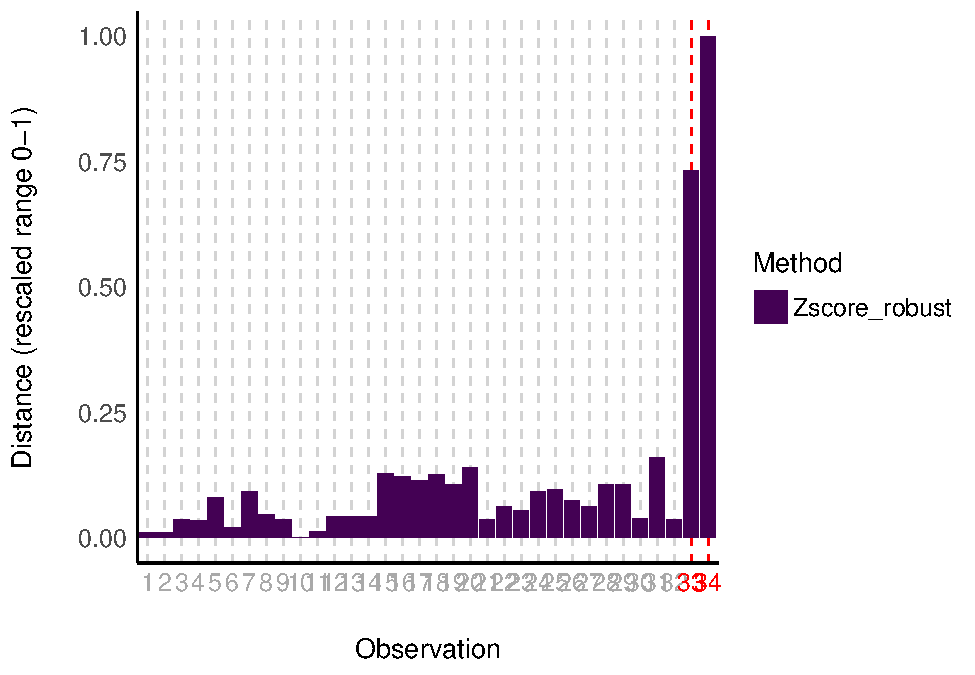
\includegraphics{paper_files/figure-latex/univariate plot-1.pdf}

\hypertarget{multivariate-outliers}{%
\subsection{Multivariate Outliers}\label{multivariate-outliers}}

For multivariate outliers, it is recommended to use the Minimum
Covariance Determinant, a robust version of the Mahalanobis distance
(MCD, Leys et al., 2019). In \{performance\}'s
\texttt{check\_outliers()}, one can use this approach with
\texttt{method\ =\ "mcd"}. The MCD can be calculated as follow (Hubert
et al., 2018):

\[
MATTHS_{gohere}^{andB}
\]

\textbf{(\textbf{mattansb?} can you add some maths here; perhaps from
Hubert et al., 2018? \url{https://doi.org/10.1002/wics.1421})}

Example:

\begin{Shaded}
\begin{Highlighting}[]
\NormalTok{x }\OtherTok{\textless{}{-}} \FunctionTok{check\_outliers}\NormalTok{(data, }\AttributeTok{method =} \StringTok{"mcd"}\NormalTok{)}
\NormalTok{x}
\end{Highlighting}
\end{Shaded}

\begin{verbatim}
## 9 outliers detected: cases 7, 15, 16, 17, 24, 29, 31, 33, 34.
## - Based on the following method and threshold: mcd (18.467).
## - For variables: mpg, cyl, disp, hp.
\end{verbatim}

\begin{Shaded}
\begin{Highlighting}[]
\FunctionTok{plot}\NormalTok{(x)}
\end{Highlighting}
\end{Shaded}

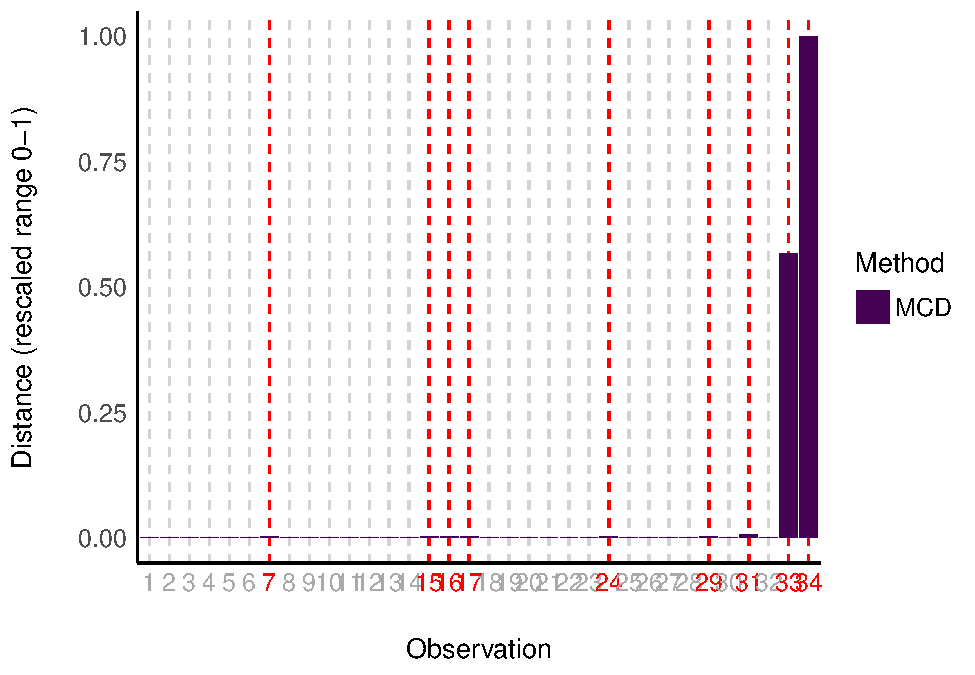
\includegraphics{paper_files/figure-latex/multivariate outliers-1.pdf}

\hypertarget{model-based-outliers}{%
\subsection{Model-Based Outliers}\label{model-based-outliers}}

{[}FIND REFERENCES TO SUPPORT MODEL-BASED OUTLIER DETECTION ABOVE ALL
OTHER METHODS!!{]}

When using linear regression models for example. In \{performance\}'s
\texttt{check\_outliers()}, one can use this approach with
\texttt{method\ =\ "cook"} (or \texttt{method\ =\ "pareto"} for Bayesian
models). The cook distance can be calculated as follow:

\[
MATTHS_{gohere}^{andB}
\]

\textbf{(\textbf{mattansb?} can you add some maths here?)}

Example:

\begin{Shaded}
\begin{Highlighting}[]
\NormalTok{model }\OtherTok{\textless{}{-}} \FunctionTok{lm}\NormalTok{(disp }\SpecialCharTok{\textasciitilde{}}\NormalTok{ mpg }\SpecialCharTok{*}\NormalTok{ hp, }\AttributeTok{data =}\NormalTok{ data)}
\NormalTok{x }\OtherTok{\textless{}{-}} \FunctionTok{check\_outliers}\NormalTok{(model, }\AttributeTok{method =} \StringTok{"cook"}\NormalTok{)}
\NormalTok{x}
\end{Highlighting}
\end{Shaded}

\begin{verbatim}
## 2 outliers detected: cases 31, 34.
## - Based on the following method and threshold: cook (0.858).
## - For variable: (Whole model).
\end{verbatim}

\begin{Shaded}
\begin{Highlighting}[]
\FunctionTok{plot}\NormalTok{(x)}
\end{Highlighting}
\end{Shaded}

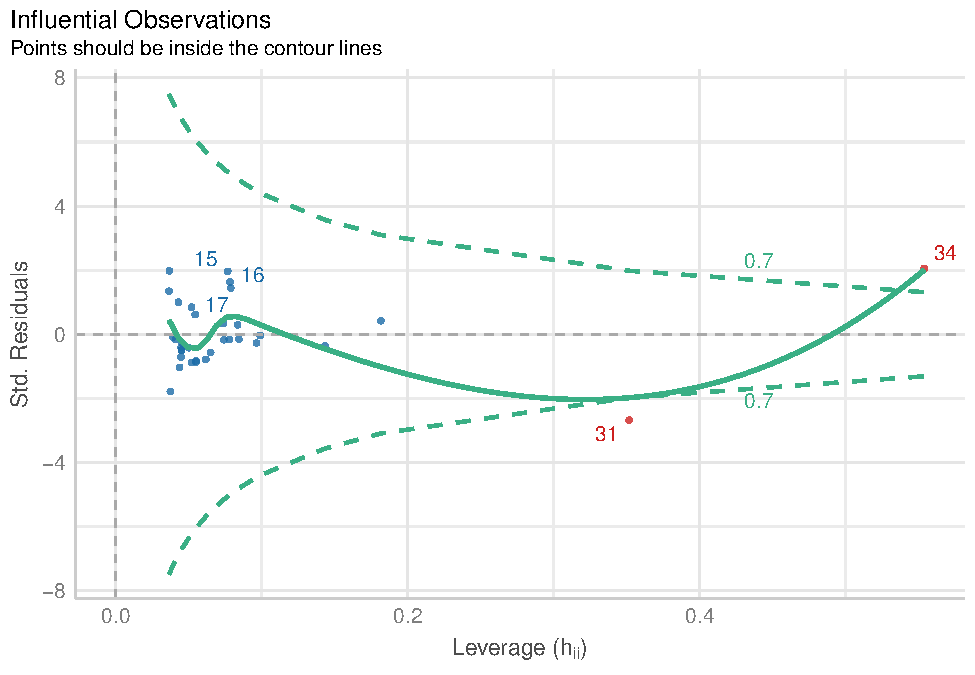
\includegraphics{paper_files/figure-latex/model-based outliers-1.pdf}

\hypertarget{multiple-methods}{%
\subsection{Multiple methods}\label{multiple-methods}}

An alternative approach suggested by easystats is to combine several
methods. This approach computes a composite outlier score, formed of the
average of the binary (0 or 1) results of each method. It represents the
probability that each observation is classified as an outlier by at
least one method. The default decision rule classifies rows with
composite outlier scores superior or equal to 0.5 as outlier
observations (i.e., that were classified as outliers by at least half of
the methods). In \{performance\}'s \texttt{check\_outliers()}, one can
use this approach by including all desired methods in the corresponding
argument.

Example:

\begin{Shaded}
\begin{Highlighting}[]
\NormalTok{x }\OtherTok{\textless{}{-}} \FunctionTok{check\_outliers}\NormalTok{(data, }\AttributeTok{method =} \FunctionTok{c}\NormalTok{(}
  \StringTok{"zscore\_robust"}\NormalTok{, }\StringTok{"iqr"}\NormalTok{, }\StringTok{"mcd"}\NormalTok{, }\StringTok{"ics"}\NormalTok{), }\AttributeTok{ID =} \StringTok{"car"}\NormalTok{)}
\NormalTok{x}
\end{Highlighting}
\end{Shaded}

\begin{verbatim}
## 3 outliers detected: cases 31, 33, 34.
## - Based on the following methods and thresholds: zscore_robust (3.09),
##   iqr (1.7), mcd (18.467), ics (0.001).
## - For variables: mpg, cyl, disp, hp.
## 
## Note: Outliers were classified as such by at least half of the selected methods. 
## 
## -----------------------------------------------------------------------------
## The following observations were considered outliers for two or more variables 
## by at least one of the selected methods: 
## 
##   Row                 car n_Zscore_robust n_IQR          n_MCD          n_ICS
## 1  33                  33               2     2 (Multivariate) (Multivariate)
## 2  34                  34               2     2 (Multivariate) (Multivariate)
## 3  31       Maserati Bora               0     1 (Multivariate) (Multivariate)
## 4   7          Duster 360               0     0 (Multivariate)              0
## 5  15  Cadillac Fleetwood               0     0 (Multivariate)              0
## 6  16 Lincoln Continental               0     0 (Multivariate)              0
## 7  17   Chrysler Imperial               0     0 (Multivariate)              0
## 8  24          Camaro Z28               0     0 (Multivariate)              0
## 9  29      Ford Pantera L               0     0 (Multivariate)              0
\end{verbatim}

\begin{Shaded}
\begin{Highlighting}[]
\FunctionTok{plot}\NormalTok{(x)}
\end{Highlighting}
\end{Shaded}

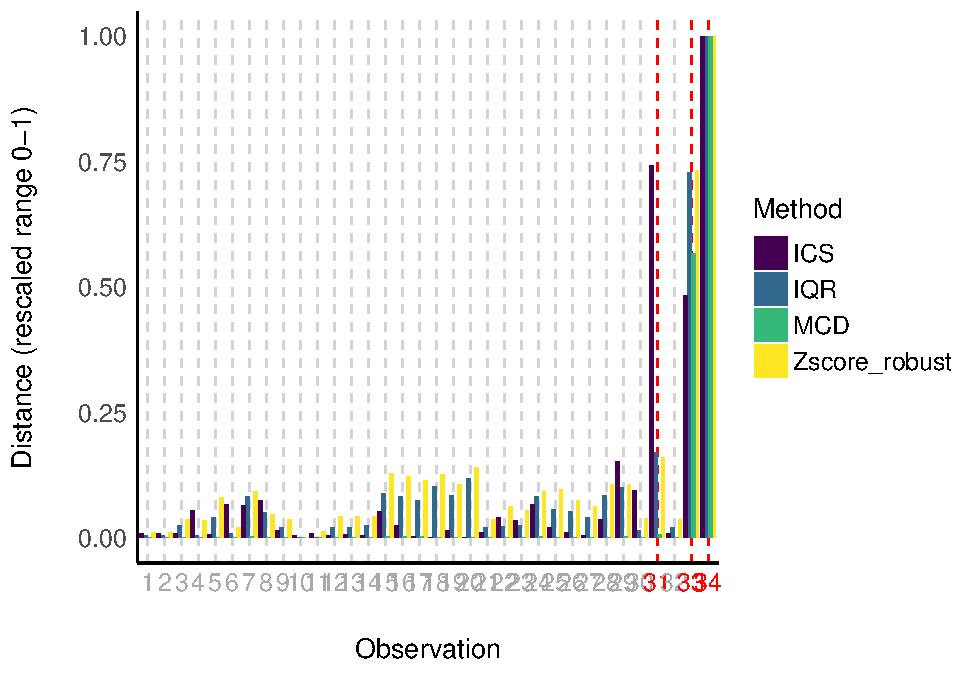
\includegraphics{paper_files/figure-latex/multimethod-1.pdf}

An example sentence for reporting the usage of the composite method
could be:

\begin{quote}
Based on a composite outlier score (see the `check\_outliers' function
in the `performance' R package, Lüdecke et al., 2021) obtained via the
joint application of multiple outliers detection algorithms ((a) median
absolute deviation (MAD)-based robust z-scores, Leys et al., 2013; (b)
interquartile range (IQR), (c) Mahalanobis minimum covariance
determinant (MCD), Leys et al., 2019; and (d) invariant coordinate
selection (ICS), Archimbaud et al., 2018), we excluded three
participants that were classified as outliers by at least half of the
methods used.
\end{quote}

\hypertarget{handling-outliers}{%
\section{Handling Outliers}\label{handling-outliers}}

We have at this point demonstrated how to identify outliers. But what
should we do with these outliers once identified? There is no
one-size-fits-all rule, as this depends on several factors. For example,
Leys et al. (2019) distinguish between error outliers, interesting
outliers, and random outliers.

\emph{Error outliers} are likely due to human error should be corrected
before data analysis or removed since they are invalid observations.
\emph{Interesting outliers} are not due to technical error and may be of
theoretical interest; it might thus be relevant to investigate them
further even though they should be removed for the current analysis of
interest. \emph{Random outliers} are assumed to be due to chance alone
and to belong to the correct distribution, therefore should be kept.

It is recommended to \emph{keep} observations which are expected to be
part of the distribution of interest, even if they are outliers (Leys et
al., 2019). However, if it is suspected that the outliers belong to an
alternative distribution, then those observations could have a large
impact on the results and call into question their robustness,
especially if significance depends on their inclusion or exclusion.

\emph{Removing} outliers can in this case be a valid strategy, and
ideally one would report results with and without outliers to see the
extent of their impact on results (assuming the study was not
preregistered with a prespecified outlier treatment plan). This approach
however can reduce statistical power. Therefore, some propose a
\emph{recoding} approach, that is, winsorization (Tukey \& McLaughlin,
1963), whereby outliers are brought back within acceptable limits (e.g.,
3 MAD). However, if possible, it is recommended to collect enough data
so that even after removing outliers, there is still sufficient
statistical power without having to resort to winsorization (Leys et
al., 2019).

We note that no matter which outlier method you use, the handling of
outliers should be specified a priori with as much detail as possible,
and ideally preregistered, to limit researchers' degrees of freedom and
therefore risks of false positives (Leys et al., 2019). This is
especially true given that interesting outliers and random outliers are
oftentimes hard to distinguish in practice. Thus, researchers should
always prioritize transparency and report exactly how many and how
outliers were handled, if possible mentioning the package, function, and
threshold used (ideally linking to the full code).

\hypertarget{winsorization}{%
\subsection{Winsorization}\label{winsorization}}

(Should we add a section on winsorization since we talk about this in
the intro/recommendations?)

\begin{Shaded}
\begin{Highlighting}[]
\NormalTok{data[}\DecValTok{33}\SpecialCharTok{:}\DecValTok{34}\NormalTok{, ]}
\end{Highlighting}
\end{Shaded}

\begin{verbatim}
##    car mpg cyl disp hp
## 33  33  42  42   42 42
## 34  34  55  55   55 55
\end{verbatim}

\begin{Shaded}
\begin{Highlighting}[]
\CommentTok{\# winsorizing using the MAD}
\FunctionTok{library}\NormalTok{(datawizard)}
\NormalTok{winsorized.data }\OtherTok{\textless{}{-}} \FunctionTok{winsorize}\NormalTok{(data, }\AttributeTok{method =} \StringTok{"zscore"}\NormalTok{, }\AttributeTok{robust =} \ConstantTok{TRUE}\NormalTok{, }\AttributeTok{threshold =} \DecValTok{3}\NormalTok{)}

\NormalTok{winsorized.data[}\DecValTok{33}\SpecialCharTok{:}\DecValTok{34}\NormalTok{, ]}
\end{Highlighting}
\end{Shaded}

\begin{verbatim}
##    car      mpg     cyl disp hp
## 33  33 37.68598 14.8956   42 42
## 34  34 37.68598 14.8956   55 55
\end{verbatim}

\hypertarget{conclusion}{%
\section{Conclusion}\label{conclusion}}

In this paper, we have showed how to investigate outliers using the
\texttt{check\_outliers} function of the \{performance\} package in
accordance with existing guidelines and good practices. We note that in
addition to using the current functions and respecting existing
recommendations, it is also important to pre-specify your plans to
manage outliers, such as with preregistration, or at the very least
justify your choices and stay consistent. Ideally, one would
additionally also report the package, function, and threshold used
(ideally linking to the full code). We hope that this paper will help
more researchers engage in good research practices while providing a
smooth experience.

\hypertarget{acknowledgments}{%
\section{Acknowledgments}\label{acknowledgments}}

\{performance\} is part of the collaborative
\href{https://github.com/easystats/easystats}{\emph{easystats}}
ecosystem. Thus, we thank the
\href{https://github.com/orgs/easystats/people}{members of easystats} as
well as the users.

\hypertarget{references}{%
\section*{References}\label{references}}
\addcontentsline{toc}{section}{References}

\hypertarget{refs}{}
\begin{CSLReferences}{1}{0}
\leavevmode\vadjust pre{\hypertarget{ref-archimbaud2018ics}{}}%
Archimbaud, A., Nordhausen, K., \& Ruiz-Gazen, A. (2018). ICS for
multivariate outlier detection with application to quality control.
\emph{Computational Statistics and Data Analysis}, \emph{128}, 184--199.
\url{https://doi.org/10.1016/j.csda.2018.06.011}

\leavevmode\vadjust pre{\hypertarget{ref-hubert2018mcd}{}}%
Hubert, M., Debruyne, M., \& Rousseeuw, P. J. (2018). Minimum covariance
determinant and extensions. \emph{Wiley Interdisciplinary Reviews:
Computational Statistics}, \emph{10}(3), e1421.
\url{https://doi.org/10.1002/wics.1421}

\leavevmode\vadjust pre{\hypertarget{ref-leys2019outliers}{}}%
Leys, C., Delacre, M., Mora, Y. L., Lakens, D., \& Ley, C. (2019). How
to classify, detect, and manage univariate and multivariate outliers,
with emphasis on pre-registration. \emph{International Review of Social
Psychology}. \url{https://doi.org/10.5334/irsp.289}

\leavevmode\vadjust pre{\hypertarget{ref-leys2013outliers}{}}%
Leys, C., Ley, C., Klein, O., Bernard, P., \& Licata, L. (2013).
Detecting outliers: Do not use standard deviation around the mean, use
absolute deviation around the median. \emph{Journal of Experimental
Social Psychology}, \emph{49}(4), 764--766.
\url{https://doi.org/10.1016/j.jesp.2013.03.013}

\leavevmode\vadjust pre{\hypertarget{ref-ludecke2021performance}{}}%
Lüdecke, D., Ben-Shachar, M. S., Patil, I., Waggoner, P., \& Makowski,
D. (2021). {performance}: An r package for assessment, comparison and
testing of statistical models. \emph{Journal of Open Source Software},
\emph{6}(60), 3139. \url{https://doi.org/10.21105/joss.03139}

\leavevmode\vadjust pre{\hypertarget{ref-simmons2011false}{}}%
Simmons, J. P., Nelson, L. D., \& Simonsohn, U. (2011). False-positive
psychology: Undisclosed flexibility in data collection and analysis
allows presenting anything as significant. \emph{Psychological Science},
\emph{22}(11), 1359--1366.
\url{https://doi.org/10.1177/0956797611417632}

\leavevmode\vadjust pre{\hypertarget{ref-tukey1963less}{}}%
Tukey, J. W., \& McLaughlin, D. H. (1963). Less vulnerable confidence
and significance procedures for location based on a single sample:
Trimming/winsorization 1. \emph{Sankhy{ā}: The Indian Journal of
Statistics, Series A}, 331--352.

\end{CSLReferences}

\end{document}
